\documentclass[First Project.tex]{subfiles}
\begin{document}

\subsection{ Σύγκλιση τροποποιήμενης μεθόδου της διχοτομήσης }

Σε αυτή την παράγραφο εκτελούμε τον αλγόριθμο της τροποποιήμενης διχοτόμησης και αναλύουμε αν συγκλίνει πάντα σε ίδιο αριθμό επαναλήψεων.
Υπενθυμίζεται ότι ο τροποποιήμενος αλγόριθμος της διχοτομήσης στην γενική περίπτωση εκτιμά την ρίζα μέσω μιας συνάρτησης παραγωγής τυχαίων
αριθμών ενώ στην συγκεκριμένη υλοποίηση του αρχείου \textlatin{\textbf{modified\_bisection.py}} οι τυχαίοι αριθμοί προέρχονται από συνεχή
ομοιόμορφη κατανομή. Εκτελούμε την συνάρτηση για την ρίζα \textbf{\textlatin{x = 2.3005}} με ορίσματα \textlatin{\textbf{a = 2.0}} και
\textlatin{\textbf{b = 2.5}} κι έχουμε τα αποτελέσματα του \textit{Σχήματος 43}

\begin{figure}[h!]
    \centering
    \captionsetup{justification=centering}
    \begin{center}
        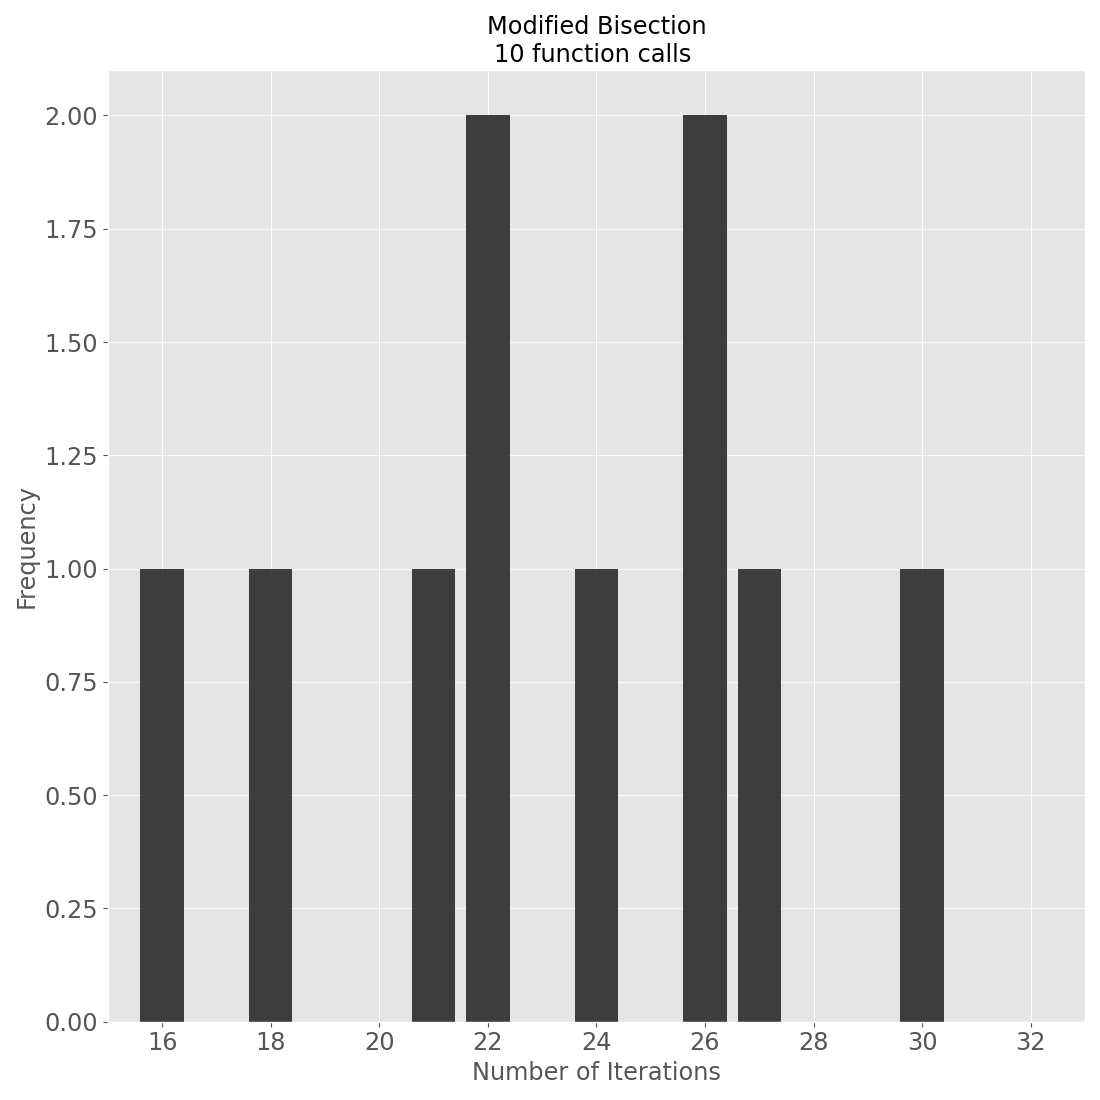
\includegraphics[scale=0.3]{modified_bisection_10_calls.png}    
        \caption{ Ιστογράμματα συχνοτήτων του αριθμού των επαναλήψεων για την τροποποιημένη μέθοδο της διχοτομήσης. }
    \end{center}
\end{figure}

Από το ιστόγραμμα του \textit{σχήματος 43} παρατηρούμε ότι ο αλγόριθμος κινείται σε αριθμούς επαναλήψεων 16 με 30 γι' αυτό το δείγμα κλήσεων της
συνάρτησης και δεν συγκλίνει πάντα σε ίδιο αριθμό επαναλήψεων. Αυτό συμβαίνει προφανώς γιατί η εκτίμηση της ρίζας σε κάθε βήμα εξαρτάται από 
την συνάρτηση παραγωγής τυχαίων αριθμών. 
\end{document}